\section{Power Injection Model (pwrmod)}  
%This is the power/current injection model Dan created for version 2.3.
%It's meant to model the `grid-following' type of inverters.
%It is included in both the non-linear and linear simulation modes of PST 4.
%There is pre-existing documentation and an example that should be condensed into this document.

The \verb|pwrmod| model was created by Dr. Trudnowski  to inject real and reactive power into a bus.
This model works with transient simulation via \verb|s_simu| and linear analysis via \verb|svm_mgen_Batch|.
\verb|pwrmod| can be used to model many devices such as wind turbines and solar plants, as well as any controls associated with such a device.

Figure \ref{fig: pwrmod BD} is a block diagram describing how power (or current) is injected into a given bus $i$.
The user constructs all devices and modeling equations in the \verb|pwrmod_dyn| function which handles the necessary equations to model the device and associated controls that perform the desired power injection.
The model must be constructed in state-space form.

\begin{figure}[H]
	\centering
	\footnotesize
	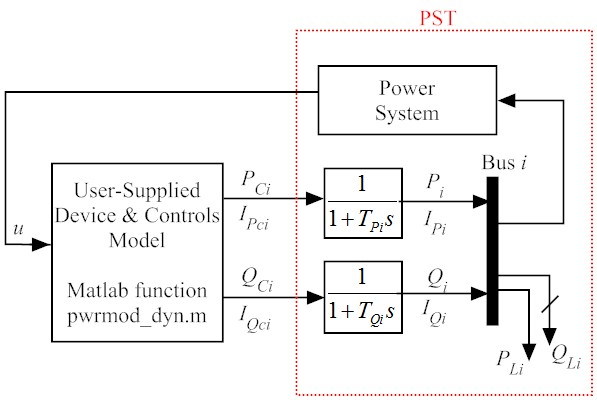
\includegraphics[width=.75\linewidth]{sections/pwrmod/BlockDiagram1}
	\caption{Block diagram of power modulation approach.}
	\label{fig: pwrmod BD}
\end{figure}%\vspace{-1 em}

The insertion of a \verb|pwrmod| model requires the target bus to be type 2 (generator type).
Additionally, the bus must be defined as constant power (for power injection) or constant current (for current injection) in the \verb|load_con|.
An example of defining bus 2 for a power injection model, and bus 3 for a current injection model using \verb|pwrmod| is shown in Listing \ref{lst: pwrmod example}.
Other examples of \verb|pwrmod| are described in Section \ref{sec: pwrmodExamples}.


\begin{lstlisting}[caption={PWRMOD Definition Example},label={lst: pwrmod example}]
\end{lstlisting}\vspace{-2 em}
\begin{minted}[
		frame=lines,
		framesep=2mm,
		baselinestretch=1.2,
		bgcolor=gray!13,
		fontsize=\footnotesize,
	%	linenos,
		breaklines
				]{MATLAB}
%% pwrmod_con format
% col 1       bus number
% col 2       real-power time constant (Tp)
% col 3       max real-power modulation (pu on system base)
% col 4       min real-power modulation (pu on system base)
% col 5       reac-power time constant (Tq)
% col 6       max reac-power modulation (pu on system base)
% col 7       min reac-power modulation (pu on system base)

pwrmod_con=[...
%bus  T    Pmax Pmin  Tq   Qmax  Qmin
  2   0.05 1    -1    0.05  1     -1; 
  3   0.05 1    -1    0.05  1     -1];

% non-conforming load
% col 1       bus number
% col 2       fraction const active power load
% col 3       fraction const reactive power load
% col 4       fraction const active current load
% col 5       fraction const reactive current load

load_con = [...
%bus Pcont Qconst P_Icont Q_Iconst
  2   1     1     0       0;    % Modulation bus for power injection
  3   0     0     1       1;];  % Modulation bus for current injection
\end{minted}
